
\section{Inference with unknown exposure status}

\paragraph{}For the known exposure status of an individual, we have shown that \textbf{Algorithm~\ref{alg:metropolis_hastings_inf}} can recover the individual-level infection status, a population-level correlate of protection and the underlying antibody kinetics for two different correlate of protection assumptions and three different levels of individual-level kinetics variability. In practice, this algorithm is unlikely to be useful as the individual-level exposure state is unknown. In this section, we will expand on this algorithm for the case when exposure status is unknown throughout the serosurvey. 

\subsection{Overview}

\paragraph{}In the case where the exposure status of each individual, $j$, is unknown, we must now infer their exposure state $E_j \in \{0, 1\}$ and the time of exposure given they are exposed $0 \leq E_j^\tau \leq 120$. In the case where $E_j = 0$, the likelihood is as derived in \textbf{Equation~\ref{ll:1E0}}. However, in the case where $E_j = 1$, the likelihood contains an additional dependencies:

\begin{equation}
L_{E_j = 1}(Z_{j}| I_j, E_j^\tau, \theta) = \prod_{t \in T_j}P_{obs}(Z_{j,t}|X_{j,t}, \sigma)P_{cop}(I_j \mid  E^\tau_{j}, \theta)
\end{equation}

where $X_{j,t} =P_{ab}( I_j,  E_j^\tau, \theta_{ab}, Z^0_i) $.

\subsubsection{Likelihood and priors}

\paragraph{}Let $\mathbf{E} = \{E_0, E_1, \dots, E_{M}\}$ be a vector describing the exposure status of each individual, let $\mathbf{E^{\tau}} = \{E^{\tau}_0, E^{\tau}_1, \dots, E^{\tau}_{n_\mathbf{E}}\}$ be a vector describing the exposure times for each exposed individual. The likelihood of this system is similar to before:

\begin{equation}
\mathcal{L}(\mathbf{Z} | \theta, \mathbf{E}, \mathbf{E^\tau}, \mathbf{I}) = \prod_{j \in \mathbf{E_0}}L_{E_j = 0}(Z_{j}| \theta) \prod_{j \in \mathbf{E_1}}L_{E_j = 1}(Z_{j}| I_j, E_j^\tau, \theta) 
\end{equation}

\paragraph{}We now must additionally define priors for $\pi(\mathbf{E})$ and $\pi(\mathbf{E^{\tau}})$. Similar to $\pi(\mathbf{I})$ we define the prior distribution for  $\pi(\mathbf{E})$ to be a Beta Binomial distribution: $\pi(\mathbf{E}) = \text{BetaBinomial}(n_{\mathbf{E}}| M, 1, 1)$, which is equal to $1/M$ for all $0 \leq n_{\mathbf{E}} \leq M$. For $\pi(\mathbf{E^{\tau}})$, we assume that each element $E_j^\tau \in \mathbf{E^{\tau}}$ has a prior given by $P_t$ such that $\pi(\mathbf{E^{\tau}}) = \prod_{j = 1}^{n_\mathbf{E}} P_t(E_j^\tau)$. The priors for $\pi(\theta)$ and $\pi(\mathbf{I})$ are as described in \textbf{Section 3}. 

\paragraph{}Consequently, we sample from the posterior distribution

\begin{equation}
P(\theta, \mathbf{E}, \mathbf{E^\tau}, \mathbf{I} | \mathbf{Z}) \propto \mathcal{L}(\mathbf{Z} | \theta, \mathbf{E}, \mathbf{E^\tau}, \mathbf{I})\pi(\theta)\pi(\mathbf{E})\pi( \mathbf{E^\tau})\pi(\mathbf{I})
\end{equation}


\paragraph{}If we use a \textbf{Algorithm~\ref{alg:metropolis_hastings_inf}} or any Metropolis Hasting algorithm to infer the exposure status and exposure time, we run into a problem. The number of parameters in the posterior distribution changes according to whether an individual is exposed, as those who are exposed, have parameters $I_j$ and $E^\tau_j$ to infer, whereas an individual who is not exposed has neither. Therefore, regardless of the proposal distribution we choose for inferring $\mathbf{E}$, we cannot use the existing algorithm highlighted in \textbf{Algorithm~\ref{alg:metropolis_hastings_inf}} as the detailed balance condition now fails. 


\subsection{The Reversible-Jump MCMC}
The Reversible Jump Markov Chain Monte Carlo (RJ-MCMC) algorithm\cite{Green1995-kh} is a Bayesian statistical method designed for model selection in situations where the number of model parameters can vary. It achieves this by introducing a stochastic mechanism that proposes moves between different models, including adding or removing parameters. The idea is to use a Metropolis-Hastings step to evaluate the acceptance probability of these proposed model changes, ensuring that the Markov chain explores the posterior distribution over both model parameters and model structures. 

\subsubsection{Mathematical overview}

\paragraph{}Let $\{k \in \mathcal{K}\}$ denote a collection models and  $\theta_k$ be the parameter space of model $k$. A full Bayesian model for inferring $k$ and $\theta_k$ can be written:

$$p(k)p(\theta_k|k)p(Z| k, \theta_k) $$

where $p(k)$ is the prior probability that model $k$ is chosen, $p(\theta_k|k)$ is the prior distribution for parameters $\theta_k$ in model $k$, and $p(Z| k, \theta_k) $ is the likelihood for the observed data for model $k$. We wish to build a Markov chain Monte Carlo algorithm to sample from the stationary distribution: 

\begin{equation}
P(\theta_k, k | Z) \propto p(k)p(\theta_k|k)p(Z | \theta_k, k)
\end{equation}

However, as the dimensions of vector $\theta_k$ change as we switch between models with different dimensions, there is no way obvious way to define $Q$ and $\alpha$ such that the detailed balance condition (\textbf{Equation~\ref{eq:db}}) is met. That is, the posterior density for the proposal state cannot be the same as the current density as the dimensions have changed. Therefore, the sampler is not converging to a single posterior distribution. 

\paragraph{}The RJ-MCMC proposes a solution to this issue \cite{Green1995-kh}. The idea is to augment both the current state and the proposed state with sampled parameters, define a bijection between these two augmented spaces, and then redefine $\alpha$ such that the detailed balance condition holds.  Let $x = (k, \theta_k)$ denote the model number $k$ and $\theta_k$ the parameters associated with model $k$ ($\theta_k \in \mathbb{R}^{d_k}$) then define the proposed state as $x' = (k', \theta_{k'})$, with $\theta_k \in \mathbb{R}^{d_{k'}}$). We write the proposal $Q(x' | x)$, the probability of moving to state $x'$ from state $x$ in the form

\begin{equation}
 Q(x'| x) = Q\left((k', \theta_{k'}) | (k, \theta_k) \right) = q_X(  \theta_{k'} |  \theta_k, k', k) \cdot q_k(k' | k)
\end{equation}

where $q_k(k' | k)$ is  the probability of selecting model $k'$ from model $k$ and $q_X$ the probabiltiy of sampling $\theta_{k'}$ given current parameters $\theta_k$ and with known  $k$, and known proposed model $k'$. The challenge with $q_X$ is that we must adjust for the change in dimensions of the parameter space of $\theta_{k'}$ compared to $\theta_k$ (i.e $d_k \neq d_{k'}$). To do this, we sample auxiliary variables to match the dimensions and define a bijection between the augmented spaces. Thus if $d_k \neq d_{k'}$, we generate a random variables of length $s$, $\mathbf{u} = (u_1, \dots, u_s) \sim q_1(\mathbf{u})$ and one of length $s'$, $\mathbf{u'} = (u'_1, \dots, u'_s) \sim q_2(\mathbf{u}')$ such that $d_{k'} + s'= d_k + s$. We then define a bijection, $T$

\begin{equation}
\label{eq:T}
(\theta_{k'}, \mathbf{u'}) = T(\theta_k, \mathbf{u}) 
\end{equation}

to ensure the reversibility of the proposal distribution. 

\paragraph{}For the detailed balance condition to hold, Green\cite{Green1995-kh} shows a prospoal distribution given by

$$Q(x | x') = q_k(k|k') q_X(\theta_{k'} | \theta_k, k, k') = q_k(k|k')q_2(\textbf{u}')\left|\frac{\partial(\theta_{k'}, \textbf{u'})}{\partial(\theta_k, u)} \right|$$ 
$$Q(x' | x) = q_k(k'|k) q_X(\theta_k | \theta_{k'}, k, k') = q_k(k'|k)q_1(\textbf{u})$$ 

where $\left|\frac{\partial(\theta_{k'}, \textbf{u}')}{\partial(\theta_k, u)} \right|$ is the jacobian of the transformation $T$. Then, choosing an acceptance ratio given 
 
 \begin{equation}
 \label{eq:alpharj}
  \alpha\left(x, x'\right) = \min\left(1, \frac{P(x)q_k(k | k')q_2(\textbf{u}') }{P(x')q_k(k' | k)q_1(\textbf{u}) }\cdot\left|\frac{\partial(\theta_{k'}, \textbf{u'})}{\partial(\theta_k, \mathbf{u})} \right|\right)
 \end{equation}


ensures the stationary distribution chain samples:

\begin{equation}
P(\theta_k, k | Z) \propto p(k)p(\theta_k|k)p(Z | \theta_k, k)
\end{equation}

A general form of the RJ-MCMC then follows \textbf{Algorithm~\ref{alg:rjmcmc_A}}.

\begin{algorithm}[H]
\caption{Reversible-Jump MCMC Algorithm}
\label{alg:rjmcmc_A}
\begin{algorithmic}[1]
    \State Chose a model $k$
    \State Initialize the chain with an initial state $\theta^{(0)}_{k}$
    \For{$i = 1$ to $N$}
         \State Sample model $k' \sim q(\cdot | k^{(i)})$
         \State Sample $\mathbf{u} \sim q_2(\textbf{u})$
	\State Set $(\theta_{k'}, \mathbf{u'}) = T(\theta_k^{(i)}, \mathbf{u})$
        \State Compute the acceptance ratio:
        \[
        \alpha \left((k^{(i)}, \theta_k^{(i)}), (k', \theta_{k'})) \right) = \min\left(1, \frac{P\left(k', \theta_{k'} | \mathbf{Z}\right)q(k^{(i)}|k')q_{2}(\mathbf{u}')}{P\left(k^{(i)}, \theta^{(i)}_{k} | \mathbf{Z}\right)q(k' | k^{(i)})q_{1}(\textbf{u})} \cdot \left| \frac{\partial(\theta_{k'}, \textbf{u}')}{\partial(\theta_k^{(i)}, \textbf{u})}\right| \right)
        \]
        \State Generate a uniform random number $u$ from the interval $[0, 1]$
        \If{$u \leq \alpha$}
            \State Accept the candidate state: $k^{(i + 1)} \leftarrow k'$ and  $\theta^{(i+1)} \leftarrow \theta_{k'}$
        \Else
            \State Reject the candidate state:$k^{(i + 1)} \leftarrow k^{(i)}$ and  $\theta^{(i+1)} \leftarrow \theta^{(i)}$
        \EndIf
    \EndFor
\end{algorithmic}
\end{algorithm}



\subsection{Application of RJ-MCMC to serological data}
\paragraph{}\textbf{Algorithm~\ref{alg:rjmcmc_A}} is a general framework for jumping from a model $k$ with a parameter values $\theta_k \in \Theta_k$ and another model $k'$ with a parameter values $\theta_{k'} \in \Theta_{k'}$. For our serological inference, our model $k$, represents different elements of the exposure state vector $\mathbf{E} = \{E_0, E_1, \dots, E_{n_\mathbf{E}}\}$ be the number of exposed individuals and $n_\mathbf{E_0} = M - n_\mathbf{E}$ be the number of non-exposed individuals in model $k$). For a given exposure vector $\mathbf{E}_k$, we define three different possible ways to sample a new exposure state vector, $\mathbf{E'}$ in our RJ-MCMC algorithm: a birth move (adding a new exposure), death move (remove an existing exposure), and parameter updating (exposure state remains the same)\cite{Liang2010-oz}. 

\subsubsection{Birth move}

\paragraph{}For a given exposure vector $\mathbf{E}$, a birth move generates a new exposure vector $\mathbf{E'}$, by randomly selecting a non-exposed individual and changing their exposure status from $E_j = 0 \rightarrow E'_j = 1$ and appending it to $\mathbf{E}$. We can derive an expression for $q_k(k' | k)$ by separating into the probability that a birth move is selected at model $k$, $q_{birth}(k' |k)$ and the probability of choosing individual $j$ uniformly from the non-exposed individuals:

\begin{equation}
q_k(k' | k) = q_{birth}(k' |k)\cdot \frac{1}{n_{\mathbf{E_0}}}
\end{equation}

\paragraph{}To understand how to evaluate $q_2(\mathbf{u}'), q_1(\mathbf{u})$, consider the change in likelihood for an individual $j$ who is chosen to be exposed:
\begin{equation}
\prod_{t \in T}P_{obs}(Z_{j,t}|Z^0_{j}, \sigma)  \rightarrow  \prod_{t \in T}P_{obs}(Z_{j,t}|X_{j,t}, \sigma)P_{cop}(I_j \mid Z^0_{j}, \theta)P_t(E_j^t)
\end{equation}

with the likelihood function staying the same for all other individuals. By changing the exposure state for individual $j$, the likelihood now depends on two parameters not in the previous likelihood: the timing of the exposure $E^\tau_j$ and their infection status $I_j$. In the notation of the previous section, it is convenient to define $\mathbf{u} = (E^\tau_j, I_j)$. Therefore, we must define a sampling procedure for $\mathbf{u}$ and a probability density function $q_1(\mathbf{u})$ (Note as $d_{k'} > d_k$, we can assume $\mathbf{u'}$ is empty).  For $E^\tau_j$, we sample from the probability density function for the timing $P_t(\cdot)$, and for the infection status, we sample from $P_{cop}(\cdot | Z_j^0, \theta_{cop})$ (see \textbf{Equation~\ref{eq:ll_cop}}). This sampling procedure results in a proposed sample which is in the proposed parameter space $\Theta_{k'}: (\theta_k, E^\tau_j, I_j) = \theta_{k'} \in \Theta_{k'}$. Consequently, we can choose the identify function for the required bijection $T$ in \textbf{Equation~\ref{eq:T}}, which means the Jacobian is equal to 1.

\paragraph{}With this sampling proposal, we can then evaluate $q_1(\mathbf{u})$ through likelihood functions for each of $I_j$ and $E^\tau_j$:

\begin{equation}
q_1(\mathbf{u}) = q_1(E^\tau_j, I_j) = P_{cop}(I_j | E_j^\tau, \theta_{cop})P_t(E^\tau_j)
\end{equation}

\paragraph{}Now let us consider the reverse move, which is from the proposed model $k'$ moving back to the model $k$. For this move, we randomly select one person from the proposed exposure state $\mathbf{E'}$ and change their exposure state from $E_j = 1 \rightarrow E'_j = 0$. Similar to above, we derived an expression for $q_k(k | k')$ by separating into the probability that an inverse birth move is selected at model $k$, $q_{birth}(k |k')$ and the probability of choosing individual $j$ uniformly from the exposed individuals of $\mathbf{E}'$:

\begin{equation}
q_k(k | k') = q_{birth}(k |k')\cdot \frac{1}{1 + n_{\mathbf{E}}}
\end{equation}


\paragraph{}In this move, we are removing the parameters $E_j^\tau$ and $I_j$ from $\theta_{k'}$. After this, we are left with $\theta_k \in \Theta_k$, so we do not need to sample new variables to generate samples from $\Theta_k$. Thus $\mathbf{u}'$ is empty and  $q_2(\mathbf{u}') = 1$. The acceptance ratio (\textbf{Equation~\ref{eq:alpharj}}) for a birth move, where our current state is $k = \{\theta, \mathbf{E}, \mathbf{E^\tau}, \mathbf{I}\} \rightarrow k' = \{\theta, \mathbf{E}', \mathbf{E^\tau}', \mathbf{I}'\}$ is updated according to a uniformed sampled non-exposed individual $j$:

\begin{equation}
\label{acc:birth}
\alpha(k, k') = \min\left(\frac{P(\theta, \mathbf{E}^{\prime}, \mathbf{E^\tau \prime}, \mathbf{I}^{\prime}, | \mathbf{Z})q_{birth}(k|k^{\prime})n_{\mathbf{E_0}}}{P(\theta, \mathbf{E}, \mathbf{E^{\tau \prime}}, \mathbf{I}, | \mathbf{Z})P_{cop}(I_{j}^{\prime} | E_{j}^{\prime}, \theta_{cop})P_t(E^{\tau \prime}_j )q_{birth}(k^{\prime} |k)(n_{\mathbf{E}} + 1)} \right)
\end{equation}


\subsubsection{Death move}


\paragraph{}For a given exposure vector $\mathbf{E}$, a death move generates a new exposure vector $\mathbf{E'}$, by randomly selecting an exposed individual and changing their exposure status from $E_j = 1 \rightarrow E'_j = 0$ therefore removing it from $\mathbf{E}$. We can derive an expression for $q_k(k' | k)$ by separating into the probability that a death move is selected at model $k$, $q_{death}(k' |k)$ and the probability of choosing individual $j$ uniformly from the exposed individuals:

\begin{equation}
q_k(k' | k) = q_{death}(k' |k)\cdot \frac{1}{n_{\mathbf{E}}}
\end{equation}

The reverse probability $q_k(k^{\prime} | k)$ is equivalent to a 'birth' move, that is the probability of sampling a non-exposed person in $\mathbf{E}'$, or 

\begin{equation}
q_k(k | k') = q_{death}(k | k')\cdot \frac{1}{1 + n_{\mathbf{E_0}}}
\end{equation}


\paragraph{}To understand how to evaluate $q_1(\mathbf{u)}, q_2(\mathbf{u}')$, consider the change in likelihood for an individual $j$ who is chosen to be exposed:
\begin{equation}
 \prod_{t \in T}P_{obs}(Z_{j,t}|X_{j,t}, \sigma)P_{cop}(I_j \mid  Z^0_{j}, \theta)P_t(E_j^\tau) \rightarrow \prod_{t \in T}P_{obs}(Z_{j,t}|Z^0_{j}, \sigma) 
\end{equation}

with the likelihood function staying the same for all other individuals. By changing the exposure state for individual $j$, the likelihood now depends on two fewer parameters than were in the previous likelihood for $k'$: the timing of the exposure $E^\tau_j$ and their infection status $I_j$. Therefore, by using the same argument as in the 'birth move' section, defining $q_1(\mathbf{u}) = 1$ and $q_2(\mathbf{u}') = F_t(E^\tau_j)F_{cop}(I_j | E_j^\tau, \theta_{cop})$, we can take the identity bijection as sample a value in state $\theta' \in \Theta'$ directly.  The acceptance ratio (\textbf{Equation~\ref{eq:alpharj}}) for a death move, where our current state is $k = \{\theta, \mathbf{E}, \mathbf{E^\tau}, \mathbf{I}\} \rightarrow k' = \{\theta, \mathbf{E}', \mathbf{E^\tau}', \mathbf{I}'\}$ is updated according to a uniformed sampled exposed individual $j$:

\begin{equation}
\label{acc:death}
\alpha(k, k^{\prime}) = \min\left(\frac{P(\theta, \mathbf{E}^{\prime}, \mathbf{E^{\tau}}^{\prime}, \mathbf{I}, | \mathbf{Z})P_{cop}(I_{j} | E_{j}, \theta_{cop})P_t(E^\tau_j)q_{death}(k|k^{\prime})n_{\mathbf{E}}}{P(\theta, \mathbf{E}, \mathbf{E^{\tau}}, \mathbf{I}, | \mathbf{Z})q_{death}(k^{\prime}|k)(n_{\mathbf{E_0}} + 1)} \right)
\end{equation}

\subsubsection{Parameter updating}


\paragraph{}In this case, $\mathbf{E_i} = \mathbf{E'}$, that is the exposure vector remains unchanged, with probability $q_{par}(k|k)$. Therefore, the detailed balanced conditions are met without dimensional adjustment. In this case, we can use sample values for $\theta$ and $\mathcal{I}$ and use the acceptance ratio highlighted in Algorithm~\ref{alg:rjmcmc_A}.

\paragraph{Note on $q_{birth}$, $q_{death}$, $q_{par}$:} We can select values $q_{birth}(k' | k)$ and $q_{death}(k' | k)$ which simplify the expression in the acceptance ratios in \textbf{Equation~\ref{acc:birth}} and \textbf{Equation~\ref{acc:death}}. If $k$ is such that $n_{\mathbf{E}} = 0$, then select we choose $q_{par} = 1/3$ and $q_{birth} = 2/3$. If  $n_{\mathbf{E}} = M$, then we choose $q_{par} = 1/3$ and $q_{death} = 2/3$. Otherwise, we  $q_{birth}(k' | k) = q_{death}(k' | k) = q_{par} = 1/3$ for all $k'$. Choosing these values means that the values of $q_{birth}$, $q_{death}$, and $q_{par}$ cancel in all acceptance ratios (\textbf{Equation~\ref{acc:birth}} and \textbf{Equation~\ref{acc:death}}) for all values of $k'$ given $k$.

\paragraph{} An algorithm describing the Birth-Death RJ-MCMC algorithm for this data is given in \textbf{Algorithm~\ref{alg:rjmcmc_B}}.

\begin{algorithm}[H]
\caption{Birth-Death Reversible Jump MCMC Algorithm}
\label{alg:rjmcmc_B}
\begin{algorithmic}[1]
    \State Chose a model $k$ and initialize the chain with an initial states $\theta^{(0)}_{k}$, $\mathbf{E^{(0)}}$, $\mathbf{E^{\tau, (0)}}$ and $\mathbf{I^{(0)}}$. If $0 < n_\mathbf{E} < M$, then $p_{birth} = p_{death} = p_{par} = 0.33$; if $n_\mathbf{E} = 0$, $p_{birth} = 0.67, p_{par} = 0.33, p_{death} = 0$; if $n_\mathbf{E} = M$, $p_{death} = 0.67, p_{par} = 0.33, p_{birth} = 0$.
    \For{$i = 1$ to $N$}
    	\State $u_1 \sim \mathcal{U}(0, 1)$  
	 \If{$u_1 \leq p_{birth}$}
	 	\State \textit{Birth move}. Select $j' \in \mathbf{E^{(i)}_0}$, set $E_{j'} = 1$, sample $E^\tau_{j'} \sim P_t(\cdot)$, $I_{j'}\sim P_{cop}(\cdot | Z_{j'}^0, \theta_{cop})$ and update $\{\theta^{(i)}, \mathbf{E^{(i)}}, \mathbf{E^{\tau, (i)}}, \mathbf{I^{(i)}}\} \rightarrow \{\theta', \mathbf{E}', \mathbf{E^\tau}', \mathbf{I}'\}$. Then calculate the acceptance probability 
		$$\alpha(k^{(i)}, k') = \min\left(\frac{P(\theta', \mathbf{E}', \mathbf{E^\tau}', \mathbf{I}', | \mathbf{Z})n_{\mathbf{E_0}}}{P(\theta, \mathbf{E^{(i)}}, \mathbf{E^{\tau, (i)}}, \mathbf{I^{(i)}}, | \mathbf{Z})P_{cop}(I_{j'} | E_{j'}, \theta_{cop})P_t(E^\tau_{j'})(n_{\mathbf{E}} + 1)} \right)$$
	\ElsIf{$u_1 \leq (p_{birth} + p_{death})$}	
		\State \textit{Death move}. Select $j' \in \mathbf{E^{(i)}_1}$, set $E_{j'} = 0$ and update $\{\theta^{(i)}, \mathbf{E^{(i)}}, \mathbf{E^{\tau, (i)}}, \mathbf{I^{(i)}}\} \rightarrow \{\theta', \mathbf{E}', \mathbf{E^\tau}', \mathbf{I}'\}$. Then calculate the acceptance probability 
$$\alpha(k^{(i)}, k') = \min\left(\frac{P(\theta', \mathbf{E}', \mathbf{E^{\tau}}', \mathbf{I} | \mathbf{Z})P_{cop}(I_{j'} | E_{j'}, \theta_{cop})P_t(E^\tau_{j'})n_{\mathbf{E}}}{P(\theta, \mathbf{E^{(i)}}, \mathbf{E^{\tau, (i)}}, \mathbf{I^{(i)}}, | \mathbf{Z})(n_{\mathbf{E_0}} + 1)} \right)$$
	\Else
 	\State Sample a candidate state $\theta' \sim q_\theta(\theta^{(i)}, \psi^{(i)}_{adapt})$
    	\State Sample  $j' \in \mathbf{E^{(i)}_1}$, and then a candidate state $I'_j \sim \text{Bernoulli(0.5)}$
    	    \State Compute the acceptance ratio:
        		\[
        \alpha(k^{(i)}, k') = \min\left(1, \frac{P(\theta', \mathbf{E}', \mathbf{E^{\tau}}', \mathbf{I}'|\mathbf{Z})}{P(\theta^{(i)}, \mathbf{E^{(i)}}, \mathbf{E^{\tau, (i)}}, \mathbf{I}^{(i)}|\mathbf{Z})} \right)
        			\]
	\State Update $ \psi^{(i + 1)}_{adapt} \leftarrow \psi^{(i)}_{adapt}$
        \EndIf 
		   \State Sample $u \sim \mathcal{U}(0, 1)$
		       \If{$u \leq \alpha$}
            			\State Accept the candidate state: Let $\{\theta^{(i+1)}, \mathbf{E^{(i+1)}}, \mathbf{E^{\tau, (i+1)}}, \mathbf{I^{(i+1)}}\} \leftarrow \{\theta', \mathbf{E}', \mathbf{E^\tau}', \mathbf{I}'\}$
			\Else
				\State Reject the candidate state: Let $\{\theta^{(i+1)}, \mathbf{E^{(i+1)}}, \mathbf{E^{\tau, (i+1)}}, \mathbf{I^{(i+1)}}\} \leftarrow \{\theta^{(i)}, \mathbf{E^{(i)}}, \mathbf{E^{\tau, (i)}}, \mathbf{I^{(i)}}\}$

			\EndIf        

    \EndFor
\end{algorithmic}
\end{algorithm}

\paragraph{Note on prior distributions}As M is fixed, then $\pi(\mathbf{E}) = 1/M$ for all $0 \leq n_{\mathbf{E}} \leq M$ and thus cancels out in the acceptance ratio for the birth, death and parameter update move. $\pi(\mathbf{I})$ cancels out in the parameter updating acceptance ratio (as described in \textbf{Algorithm~\ref{alg:metropolis_hastings_inf}}. However, in the birth and death move, as $n_{\mathbf{E}}$ in the current state and $n_{\mathbf{E}'}$ is the proposed state have different values, then $\pi(\mathbf{I}) = 1/n_\mathbf{E_1} \neq  1/n_\mathbf{E_1'} = \pi(\mathbf{I}')$ no longer cancels in the ratio and must be included to ensure the detailed balance condition holds. 
We choose a non-informative for the timing of infection given exposure prior: $P_t(E_j^\tau) = 1 / 120$.

\subsubsection{Within Gibbs sampling of exposure times}

\paragraph{}\textbf{Algorihtm~\ref{alg:rjmcmc_B}} allows for efficient sampling of the $\theta$, $\mathbf{I}$, and $\mathbf{E}$. However, the timing of the exposures, $\mathbf{E^\tau}$ is not efficiently explored as it can only be changed at a birth or death move. Therefore, it is desirable that values of $\mathbf{E^\tau}$ can be explored for fixed values of $\mathbf{I}$, and $\mathbf{E}$. To do this, we modify \textbf{Algorihtm~\ref{alg:rjmcmc_B}} to allow the possibility of exploration of the $\mathbf{E^\tau}$ timings for a given model $k$ whilst $\mathbf{I}$, and $\mathbf{E}$ remain fixed. To implement this, after the candidate state has been accepted or rejected in \textbf{Algorithm~\ref{alg:rjmcmc_B}}, we then resample a proportion of the $\mathbf{E}^{tau}$, and for each individual, we sample a new time $E_{j'}^\tau$ from the proposal distribution

$$E_{j'}^{\tau} \sim q_t(E_{j}^{\tau}) $$

where we choose the proposal to be the symmetric $q_t(E_{j}^{\tau}) = \mathcal{N}(E_j^{t, (i)}, \sigma^{(i)}_j)$.  Where $\sigma^{(i)}_j$ is an adaptively updated standard deviation for the proposal for the normal, which updates according to the regime:

$$\log\left(\sigma^{(i + 1)}_j\right) = \log\left(\sigma^{(i)}_j\right) +  (1 + i)^{-0.5}*(\alpha - 0.44) $$

where $\alpha$ is the metropolis hasting ratio for $E_{j'}^{\tau}$ vs $E_j^{\tau, (i)}$.

Therefore the final RJMCMC algorithm (\textbf{Algorithm~\ref{alg:rjmcmc_C}}) which effectively samples values from $\theta$, $\mathbf{E}$, $\mathbf{E_\tau}$, $\mathbf{I}$. 

\begin{algorithm}[H]
\caption{Efficient Birth-Death Reversible Jump MCMC Algorithm}
\label{alg:rjmcmc_C}
\begin{algorithmic}[1]
 \State Chose a model $k$ and initialise the chain with an initial states $\theta^{(0)}_{k}$, $\mathbf{E^{(0)}}$, $\mathbf{E^{\tau, (0)}}$ and $\mathbf{I^{(0)}}$.
    \For{$i = 1$ to $N$}
    	\State Update $\{\theta^{(i + 1)}, \mathbf{E^{(i + 1)}}, \mathbf{E^{\tau, (i + 1)}}, \mathbf{I^{(i + 1)}}\}$ according to \textbf{Algroithm~\ref{alg:rjmcmc_B}}.
	    \For{$k = 1$ to $N_k$}
        \State Select $j' \in N_{E = 1}$ and resample from the proposal $E_{j'}^{\tau} \sim \mathcal{N}\left(E_{j}^{\tau, (i)}, \sigma^{(i)}_{j}\right)$ and update $\mathbf{E^{t, (i)}} \rightarrow \mathbf{E^{t, *}}$
            \State Compute the acceptance ratio:
        		\[
        		\alpha(k^{(i)}, k^{\prime}) = \min\left(1, \frac{P(\theta^{(i)}, \mathbf{E^{(i)}}, \mathbf{E^{\tau \prime}}, \mathbf{I^{(i)}}|\mathbf{Z})}{P(\theta^{(i)}, \mathbf{E^{(i)}}, \mathbf{E^{\tau, (i)}}, \mathbf{I^{(i)}}|\mathbf{Z})} \right)
        			\]
  \State Sample $u \sim \mathcal{U}(0, 1)$
	\If{$u \leq \alpha$}
            	\State Accept the candidate state: $\mathbf{E^{\tau, (i + 1)}}  \leftarrow \mathbf{E^{\tau\prime}} $
        \Else
            \State Reject the candidate state:$\mathbf{E^{\tau, (i + 1)}}  \leftarrow \mathbf{E^{\tau, (i)}} $
        \EndIf 
        \State Update $\log\left(\sigma_{j'}^{(i_k + 1)}\right) \leftarrow \log\left(\sigma_{j'}^{(i_k)}\right) + (1 +  i_k)^{-0.5}(\alpha - 0.44)$
        \State $i_{k + 1} \leftarrow i_k + 1$
            \EndFor
    \EndFor
\end{algorithmic}
\end{algorithm}


\subsubsection{Summary}
\paragraph{}Through \textbf{Algorithm~\ref{alg:rjmcmc_C}} we define an efficient sampling procedure for the state space $k = \{\theta, \mathbf{E}, \mathbf{E^\tau}, \mathbf{I}\}$ within one single framework. This allows us to infer the exposure state, infection state, exposure and infection timings across the epidemic, the correlates of protection and the antibody kinetics function. We show the ability of this procedure to recover our simulated data displayed in the next section.

\subsection{Simulation recovery }
\paragraph{}After running \textbf{Algorithm~\ref{alg:rjmcmc_C}}, we plot the posterior samples, $\hat{\theta}$, $\hat{\mathbf{I}}$,  $\hat{\mathbf{E}}$, and  $\hat{\mathbf{E}^\tau}$ and compare with the simulated parameters.

\subsubsection{Exposure state recovery}
\paragraph{} \textbf{Algorithm~\ref{alg:rjmcmc_C}} can predict and recover the population-level exposure rates, but struggles on the individual level (\textbf{Figure~\ref{fit2:exp}}). For those exposed and infected, the exposure rate is consistently recovered, except when the pre-infection titre is greater than 3.3, in which the boosting is completely attenuated. At these high titres, infection, exposed and not infected, and non-exposure all have the same antibody kinetics (i.e. unchanged titre throughout the study), and thus, the model cannot differentiate between these exposure-infection states on an individual level. The expectation of the posterior values $\mathbb{E}[\hat{E}] = 0.5$, implying no preference between a positive or negative state. The model also cannot identify which individuals are exposed and not infected and which are not exposed for all titre values. This is unsurprising, as both these individuals have the same antibody kinetics regardless of pre-infection titre (i.e. unchanged throughout the study). In the case of a correlation of protection with a logistic function, there is some inference on the posterior probability of exposure $\hat{E}$ given pre-infection titre. At low titre values, it is unlikely an individual is exposed and not infected, as the probability of infection given exposure is high. Therefore, the model infers these individuals are unlikely to have been exposed $\mathbb{E}[\hat{E}] < 0.5$. This COP influence causes the increasing value of the $\mathbb{E}[\hat{E}]$ for each individual as the titre increases in \textbf{Figure~\ref{fit2:exp}}. Finally, the number of exposed individuals is approximately recovered for all six models. 

\begin{figure}[H]

    \centering
    \begin{subfigure}{0.31\textwidth}
        \centering
        \includegraphics[width=\textwidth]{\myimagepath/outputs/fits/cesNoCOP/inferExp/figs/obs_0.1/exposure_recov.png}
        \caption{No COP, 10\% observation error \label{fit1:inf}}
    \end{subfigure}
    \begin{subfigure}{0.31\textwidth}
        \centering
        \includegraphics[width=\textwidth]{\myimagepath/outputs/fits/cesNoCOP/inferExp/figs/obs_0.3/exposure_recov.png}
        \caption{No COP, 30\% observation error}
    \end{subfigure}
    \begin{subfigure}{0.31\textwidth}
        \centering
        \includegraphics[width=\textwidth]{\myimagepath/outputs/fits/cesNoCOP/inferExp/figs/obs_0.5/exposure_recov.png}
        \caption{No COP, 50\% observation error}
    \end{subfigure}
    
  \begin{subfigure}{0.31\textwidth}
        \centering
        \includegraphics[width=\textwidth]{\myimagepath/outputs/fits/cesCOP/inferExp/figs/obs_0.1/exposure_recov.png}
        \caption{ COP, 10\% observation error}
    \end{subfigure}
    \begin{subfigure}{0.31\textwidth}
        \centering
        \includegraphics[width=\textwidth]{\myimagepath/outputs/fits/cesCOP/inferExp/figs/obs_0.3/exposure_recov.png}
        \caption{ COP, 30\% observation error}
    \end{subfigure}
    \begin{subfigure}{0.31\textwidth}
        \centering
        \includegraphics[width=\textwidth]{\myimagepath/outputs/fits/cesCOP/inferExp/figs/obs_0.5/exposure_recov.png}
        \caption{ COP, 50\% observation error}
    \end{subfigure}
    
    \caption{Simulation recovery of exposure status $\hat{E}$ and epidemic curve for two COP models (top: No COP, bottom: logistic COP) and three different levels antibody kinetics variability (10\%, 30\%, 50\%) \label{fit2:exp}}
\end{figure}

\subsubsection{Exposure times recovery}
\paragraph{} \textbf{Algorithm~\ref{alg:rjmcmc_C}} can recover the exposure times under specific conditions. The posterior of the exposure times for individual $j$ is given by $\hat{E^\tau_j}$ and plotted with the simulated exposure time in \textbf{Figure~\ref{fit2:exp} } by their exposure status. For those infected, the model can reasonably recover the exposure times for each individual, though as the antibody kinetics variability increases, the exposure time becomes less recoverable. For those who are exposed and not infected, the model cannot infer the exposure time as there is an inference method for this in the likelihood (i.e. exposure time is determined by antibody kinetics, and antibody kinetics remain unchanged for those exposed and not infected). Therefore the inferred exposure time for this individual is the same as the prior entered into the model. For all six models, the epidemic curve is reasonably recovered (\textbf{Figure~\ref{fit2:exp}}).

\begin{figure}[H]

    \centering
    \begin{subfigure}{0.31\textwidth}
        \centering
        \includegraphics[width=\textwidth]{\myimagepath/outputs/fits/cesNoCOP/inferExp/figs/obs_0.1/exposure_time_recov.png}
        \caption{No COP, 10\% observation error \label{fit1:inf}}
    \end{subfigure}
    \begin{subfigure}{0.31\textwidth}
        \centering
        \includegraphics[width=\textwidth]{\myimagepath/outputs/fits/cesNoCOP/inferExp/figs/obs_0.3/exposure_time_recov.png}
        \caption{No COP, 30\% observation error}
    \end{subfigure}
    \begin{subfigure}{0.31\textwidth}
        \centering
        \includegraphics[width=\textwidth]{\myimagepath/outputs/fits/cesNoCOP/inferExp/figs/obs_0.5/exposure_time_recov.png}
        \caption{No COP, 50\% observation error}
    \end{subfigure}
    
  \begin{subfigure}{0.31\textwidth}
        \centering
        \includegraphics[width=\textwidth]{\myimagepath/outputs/fits/cesCOP/inferExp/figs/obs_0.1/exposure_time_recov.png}
        \caption{ COP, 10\% observation error}
    \end{subfigure}
    \begin{subfigure}{0.31\textwidth}
        \centering
        \includegraphics[width=\textwidth]{\myimagepath/outputs/fits/cesCOP/inferExp/figs/obs_0.3/exposure_time_recov.png}
        \caption{ COP, 30\% observation error}
    \end{subfigure}
    \begin{subfigure}{0.31\textwidth}
        \centering
        \includegraphics[width=\textwidth]{\myimagepath/outputs/fits/cesCOP/inferExp/figs/obs_0.5/exposure_time_recov.png}
        \caption{ COP, 50\% observation error}
    \end{subfigure}
    
    \caption{Simulation recovery of exposure and infection timtings $\hat{E^\tau}$ and epidemic curve for two COP models (top: No COP, bottom: logistic COP) and three different levels antibody kinetics variability (10\%, 30\%, 50\%) \label{fit2:exp}}
\end{figure}



\subsubsection{Infection state recovery}

\paragraph{}We also recover the infection status of each individual from the simulated data. If the set posterior samples of the infection status for individual $j$ is given by $\hat{I_j} $, then we plot the expectation $\mathbb{E}(\hat{I_j} )$ so we can assess the ability of the algorithm to recover the individual-level simulated infection status (\textbf{Figure~\ref{fit2:inf}}). As before, we find when the pre-infection titre < 3.3 log titre value that all six models considered can recover the infection status of almost all individuals. When the pre-infection titre is greater than 3.3, the attenuation of boosting for infected individuals causes no meaningful change in the antibody kinetics ($f^2_{ab}(Z, \alpha) = 0$ when $Z > 3.3$). Thus, these individuals' infections are difficult to infer serologically as their titre dynamics are equivalent to independent of their infection status. In our COP model B, we find that including the correlation of protection influences the infection status. As the inferred correlate has a low probability of infection at higher titres, this causes the $\hat{I_j}$ to be more likely to be 0 at higher titre values. 

\begin{figure}[H]
    \centering
    \begin{subfigure}{0.31\textwidth}
        \centering
        \includegraphics[width=\textwidth]{\myimagepath/outputs/fits/cesNoCOP/inferExp/figs/obs_0.1/infection_recov.png}
        \caption{No COP, 10\% observation error \label{fit1:inf}}
    \end{subfigure}
    \begin{subfigure}{0.31\textwidth}
        \centering
        \includegraphics[width=\textwidth]{\myimagepath/outputs/fits/cesNoCOP/inferExp/figs/obs_0.3/infection_recov.png}
        \caption{No COP, 30\% observation error}
    \end{subfigure}
    \begin{subfigure}{0.31\textwidth}
        \centering
        \includegraphics[width=\textwidth]{\myimagepath/outputs/fits/cesNoCOP/inferExp/figs/obs_0.5/infection_recov.png}
        \caption{No COP, 50\% observation error}
    \end{subfigure}
    
  \begin{subfigure}{0.31\textwidth}
        \centering
        \includegraphics[width=\textwidth]{\myimagepath/outputs/fits/cesCOP/inferExp/figs/obs_0.1/infection_recov.png}
        \caption{ COP, 10\% observation error}
    \end{subfigure}
    \begin{subfigure}{0.31\textwidth}
        \centering
        \includegraphics[width=\textwidth]{\myimagepath/outputs/fits/cesCOP/inferExp/figs/obs_0.3/infection_recov.png}
        \caption{ COP, 30\% observation error}
    \end{subfigure}
    \begin{subfigure}{0.31\textwidth}
        \centering
        \includegraphics[width=\textwidth]{\myimagepath/outputs/fits/cesCOP/inferExp/figs/obs_0.5/infection_recov.png}
        \caption{ COP, 50\% observation error}
    \end{subfigure}
    
    \caption{Simulation recovery of the individual infection status, $\hat{I_j}$, for two COP models (top: No COP, bottom: logistic COP) and three different levels antibody kinetics variability (10\%, 30\%, 50\%) \label{fit2:inf}}
\end{figure}

\subsubsection{Correlate of protection}

\paragraph{} \textbf{Algorithm~\ref{alg:rjmcmc_C}} performs well at ]ecovering the correlate of protection function $f_{cop}(x, \hat{\theta}_{cop})$, where $x$ is the titre value at infection and where $\hat{\theta}_{cop} = \{\hat{\beta_0}, \hat{\beta_1}\}$ are the posterior samples for $\beta_0$ and $\beta_1$. For Model A, we find that the COP curve is recovered, with the simulated line within a 50\% confidence interval of the posterior sample (\textbf{Figure~\ref{fit2:cop}}). For Model B, we find the logistic shape of the COP is recovered in the posterior samples. 

\begin{figure}[H]

    \centering
    \begin{subfigure}{0.31\textwidth}
        \centering
        \includegraphics[width=\textwidth]{\myimagepath/outputs/fits/cesNoCOP/inferExp/figs/obs_0.1/cop_recov.png}
        \caption{No COP, 10\% observation error}
    \end{subfigure}
    \begin{subfigure}{0.31\textwidth}
        \centering
        \includegraphics[width=\textwidth]{\myimagepath/outputs/fits/cesNoCOP/inferExp/figs/obs_0.3/cop_recov.png}
        \caption{No COP, 30\% observation error}
    \end{subfigure}
    \begin{subfigure}{0.31\textwidth}
        \centering
        \includegraphics[width=\textwidth]{\myimagepath/outputs/fits/cesNoCOP/inferExp/figs/obs_0.5/cop_recov.png}
        \caption{No COP, 50\% observation error}
    \end{subfigure}
    
  \begin{subfigure}{0.31\textwidth}
        \centering
        \includegraphics[width=\textwidth]{\myimagepath/outputs/fits/cesCOP/inferExp/figs/obs_0.1/cop_recov.png}
        \caption{ COP, 10\% observation error}
    \end{subfigure}
    \begin{subfigure}{0.31\textwidth}
        \centering
        \includegraphics[width=\textwidth]{\myimagepath/outputs/fits/cesCOP/inferExp/figs/obs_0.3/cop_recov.png}
        \caption{ COP, 30\% observation error}
    \end{subfigure}
    \begin{subfigure}{0.31\textwidth}
        \centering
        \includegraphics[width=\textwidth]{\myimagepath/outputs/fits/cesCOP/inferExp/figs/obs_0.5/cop_recov.png}
        \caption{ COP, 50\% observation error}
    \end{subfigure}
    
    \caption{Simulation recovery of the COP function, posterior samples plot  $f_{cop}(x, \hat{\theta}_{cop})$. We have two different COp models (top: No COP, bottom: logistic COP) and three different levels of antibody kinetics variability (10\%, 30\%, 50\%). \label{fit2:cop}}
\end{figure}




\subsubsection{Antibody kinetics}
\paragraph{} \textbf{Algorithm~\ref{alg:rjmcmc_C}} also succesfully recovers the simualted antibody kinetics. Let us plot $f^1_{ab}(s, \hat{a}, \hat{b}, \hat{c})$, the posterior predictive distribution for the antibody kinetic boosting, given posterior distributions for $ \hat{a}, \hat{b}$, and $\hat{c}$. At all three levels of kinetic uncertainty, the antibody kinetics are recovered, though increasing uncertainty weakens the accuracy of the recovered curves compared to the simulated. (\textbf{Figure~\ref{fit2:ab}}).

\begin{figure}[H]

    \centering
    \begin{subfigure}{0.31\textwidth}
        \centering
        \includegraphics[width=\textwidth]{\myimagepath/outputs/fits/cesNoCOP/inferExp/figs/obs_0.1/ab_kinetics_recov.png}
        \caption{No COP, 10\% observation error}
    \end{subfigure}
    \begin{subfigure}{0.31\textwidth}
        \centering
        \includegraphics[width=\textwidth]{\myimagepath/outputs/fits/cesNoCOP/inferExp/figs/obs_0.3/ab_kinetics_recov.png}
        \caption{No COP, 30\% observation error}
    \end{subfigure}
    \begin{subfigure}{0.31\textwidth}
        \centering
        \includegraphics[width=\textwidth]{\myimagepath/outputs/fits/cesNoCOP/inferExp/figs/obs_0.5/ab_kinetics_recov.png}
        \caption{No COP, 50\% observation error}
    \end{subfigure}
    
  \begin{subfigure}{0.31\textwidth}
        \centering
        \includegraphics[width=\textwidth]{\myimagepath/outputs/fits/cesCOP/inferExp/figs/obs_0.1/ab_kinetics_recov.png}
        \caption{ COP, 10\% observation error}
    \end{subfigure}
    \begin{subfigure}{0.31\textwidth}
        \centering
        \includegraphics[width=\textwidth]{\myimagepath/outputs/fits/cesCOP/inferExp/figs/obs_0.3/ab_kinetics_recov.png}
        \caption{ COP, 30\% observation error}
    \end{subfigure}
    \begin{subfigure}{0.31\textwidth}
        \centering
        \includegraphics[width=\textwidth]{\myimagepath/outputs/fits/cesCOP/inferExp/figs/obs_0.5/ab_kinetics_recov.png}
        \caption{ COP, 50\% observation error}
    \end{subfigure}
    
    \caption{Simulation recovery of the antibody kinetics function with posterior samples plot $f^1_{ab}(s, \hat{a}, \hat{b}, \hat{c})$. We have two different COP models (top: No COP, bottom: logistic COP) and three different levels of antibody kinetics variability (10\%, 30\%, 50\%). \label{fit2:ab}}
   \end{figure}
